%%---------- Uitvoeren testen PoC-----------------------------------------------------


\chapter{\IfLanguageName{dutch}{Testen van PoC}{Testing on PoC}}
\label{ch:test-poc}
\section{Test scenario's}
De applicatie kan zich in verschillende toestanden bevinden. De eerste toestand is wanneer de applicatie idle draait. Dit komt voor als er geen web requests binnenkomen en er achterliggend geen 'processen' lopen, zoals verwerken van data. Een tweede toestand is wanneer er wel web requests binnenkomen. Deze triggeren dataverwerking, bijvoorbeeld, in het kader van deze Proof of Concept, kan dit het ophalen en berekenen van het verbruik van een telefoonnummer zijn. De eerste toestand zal vermoedelijk minder energie verbruiken dan de tweede.\\

De verschillende scenario's dat getest zullen worden zijn als volgt:
\begin{itemize}
    \item Een idle systeem voor 10 seconden, gesimuleerd door een slaap actie (Bijlage \ref{bij_scen_1});
    \item Een systeem met 100 web requests (Bijlage \ref{bij_scen_2});
    \item Een systeem met 500 web requests (Bijlage \ref{bij_scen_3});
    \item een systeem met 2500 web requests (Bijlage \ref{bij_scen_4}).
\end{itemize}

Bij het versturen van requests worden deze evenredig verdeeld over de pagina's. Dit wil zeggen dat elke pagina, waarvan er 3 zijn, 33.33\% van de requests toegewezen krijgen. Deze scenario's worden op elke ontwikkelarchitectuur 50 keer uitgevoerd waardoor genoeg data beschikbaar is om een zo betrouwbaar mogelijk beeld te vormen over het energieverbruik van de applicatie.

\section{Automatisatie van de testen}\label{tpoc_auto_test}
Voor het minimaliseren van de invloed door gebruikersinput worden de testen geautomatiseerd. Twee bash script zijn hiervoor voorzien in bijlage \ref{bij_start_testing} en bijlage \ref{bij_call_testing}. Het eerste script heeft 2 taken. Allereerst worden alle docker omgevingen gereset om vervolgens de docker omgeving van de juiste applicatie, zijnde de monoliet of microservice, op te starten. Dit gebeurt door de correcte docker-compose containers op te starten. Vervolgens starten de metingen door het aanroepen van het tweede script. \\

Het tweede script start een PowerJoular meting op de applicatie en roept hierna een script aan die de bijhorende actie uitvoert voor elk testscenario. Na het uitvoeren van elk testscenario-script stopt de PowerJoular instantie en wordt het gemeten energieverbruik weggeschreven naar een csv-bestand. Na het wegschrijven begint het script opnieuw bij het starten van een PowerJoular instantie.\\

\section{Uitvoeren van de testen}
Om de testen te kunnen uitvoeren moeten deze scripts als executable ingesteld worden. Dit kan door het commando \textit{sudo chmod +x <script bestand>} uit te voeren op elk script. Het starten van de testen kan door het commando \textit{./autostart\_tests\_and\_analysis.sh} in de folder van de testen. Elk script zal indiceren wanneer het beëindigd is, alsook een finale melding geven dat alle data is opgeslagen in het csv-bestand. Dit is voorgesteld in figuur \ref{tpoc_script_output}.\\  
\begin{figure}[h!]
    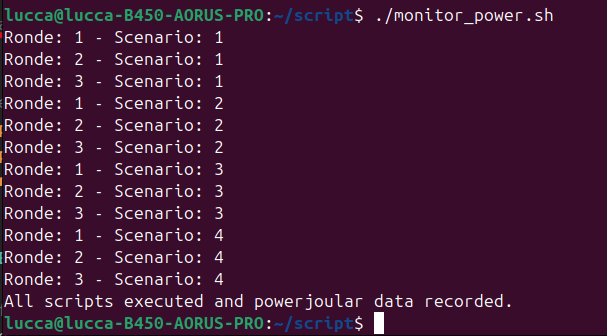
\includegraphics[scale=0.75]{tpoc_script_execution}
    \centering
    \caption{Voorbeeld scriptuitvoer testen PoC}
    \label{tpoc_script_output}
\end{figure}